\documentclass[12pt, a4paper]{report}
\usepackage{graphicx, array, amsthm, amssymb, amsmath, algorithm, algpseudocode, float, xcolor, thmtools, thmbox, matlab-prettifier, exercise}
\usepackage[english]{babel}

\makeatletter
\renewcommand\thmbox@headstyle[2]{\bfseries #1}
\makeatother
\newtheorem[style=M,bodystyle=\normalfont]{theorem}{Theorem}
\newtheorem[style=M,bodystyle=\normalfont]{corollary}{Corollary}
\newtheorem[style=M,bodystyle=\normalfont]{lemma}{Lemma}
\newtheorem[style=M,bodystyle=\normalfont]{definition}{Definition}

\definecolor{dkgreen}{rgb}{0,0.6,0}
\definecolor{gray}{rgb}{0.5,0.5,0.5}
\definecolor{mauve}{rgb}{0.58,0,0.82}
\lstset{frame=tb,
  language=Java,
  aboveskip=3mm,
  belowskip=3mm,
  showstringspaces=false,
  columns=flexible,
  basicstyle={\small\ttfamily},
  numbers=none,
  numberstyle=\tiny\color{gray},
  keywordstyle=\color{blue},
  commentstyle=\color{dkgreen},
  stringstyle=\color{mauve},
  breaklines=true,
  breakatwhitespace=true,
  tabsize=3
}


\title{Image Analysis And Computer Vision\\ \textit{Exercises}}
\author{Christian Rossi}
\date{Academic Year 2023-2024}

\begin{document}

\maketitle

\newpage

\begin{abstract}
    The topics of the course are: 
    \begin{itemize}
        \item Introduction.
        \item Camera sensors: transduction, optics, geometry, distortion
        \item Basics on Projective geometry: modelling basic primitives (points, lines, planes, conic sections, quadric surfaces) and projective spatial transformations and  projections.
        \item Camera geometry, and single view analysis: calibration, image rectification, localization of 3D models.
        \item Multi-view analysis: 3D shape reconstruction, self-calibration, 3D scene understanding.
        \item Linear filters and convolutions, space-invariant filters, Fourier Transform, sampling and aliasing. 
        \item Nonlinear filters: image morphology and morphology operators (dilate, erode, open, close), median filters.
        \item Edge detection and feature detection techniques. Feature matching and feature tracking along image sequences.
        \item Inferring parametric models from noisy data (including outliers), contour segmentation, clustering, Hough Transform, Ransac (random sample consensus). 
        \item Applications: object tracking, object recognition, classification.
    \end{itemize}
\end{abstract}

\newpage

\tableofcontents

\newpage

\chapter{Introduction to MATLAB}
    \section{Main MATLAB operators}
    To print some string it is possible to use; 
    \begin{lstlisting}[language=Matlab]
% Print the string
disp('string');
% Print the string with C-like syntax
fprintf('string\n%s %d','string',number);
    \end{lstlisting}
    The variables are created as follows: 
    \begin{lstlisting}[language=Matlab]
% Variables are created by assignements
v=3
c='k'
% Data types can be checked
whos v
% Casting to 8-bit integer
v=uint8(v)
    \end{lstlisting}
    The main data types used on MATLAB: double, uint8, and logical. The arrays are defined in the following ways: 
    \begin{lstlisting}[language=Matlab]
% A row vector
r=[1, 2, 3, 4]
% A column vector
c=[1; 2; 3; 4]
% Vectors by regular increment operator
% [start:step:end]
a = [1:2:10];
% A matrix
v=[ 1 2; 
    3 4 ]
    \end{lstlisting}
    It is possible to concatenate arrays: 
    \begin{lstlisting}[language=Matlab]
B=[v', v']
C=[v; v]        
    \end{lstlisting}
    The arrays can be divided in subarrays: 
    \begin{lstlisting}[language=Matlab]
% First row and second column 
v(1,2) 
% The second column of v
v(:,2)
% The first row of v
v(1,:) 
% Some of the columns from 2 to 4
B(:,2:4) 
    \end{lstlisting}
    Some useful mathematical operations are: 
    \begin{lstlisting}[language=Matlab]
% . means elementwise operation
[1 2 3].*[4 5 6]
[1 2 3]+5
[1 2 3]*2 
[1 2 3].*2 
[1 2 3]/2
[1 2 3]./2 
[1 2 3].^2 
% Inner product
[1 2 3]*[4 5 6]' 
% This is the matrix product, returns a matrix
[1 2 3]'*[4 5 6] 
% Functions for rounding functions
ceil(10.56)
floor(10.56)
round(10.56)
% Arithmetic functions
sum([1 2 3 4])
sum([1:4;5:8])
sum([1:4;5:8],2)
    \end{lstlisting}

    \section{Commands for images}
    The images in MATLAB are treated as matrices:
    \begin{lstlisting}[language=Matlab]
im=imread('photo.png');
% Show the image
imshow(im);
% Show two concatenated images orizontally
imshow([im im]);
% Show two concatenated images vertically
imshow([im; im]);
    \end{lstlisting}
    To plot the histogram of the various pixels it is possible to write: 
    \begin{lstlisting}[language=Matlab]
h=hist(im(:),[0: im_length]);
figure(2), stairs([0: im_length], h)
axis tight
    \end{lstlisting}
    It is possible to modify the brightness and contrast with a simple operation:
    \begin{lstlisting}[language=Matlab]
figure(1),imshow(im+50),title('50 graylevels')
figure(1),imshow(im+100),title('100 graylevels')
% contrast modify
eq=double(im-min(im(:)))/double(max(im(:))-min(im(:)))*255;
    \end{lstlisting}
    Image ranges (in the visualization) can be also controlled:
    \begin{lstlisting}[language=Matlab]
imshow(im,[-100 156]);title('more brighness');
imshow(im,[0 156]);title('more brighness and contrast');
imshow(im,[ 100 256]);title('less brighness, more contrast');
imshow(im,[ 100 356]);title('less brighness');
    \end{lstlisting}
    The gamma correction is done in this way: 
    \begin{lstlisting}[language=Matlab]
for gamma= [.04 .1 .2 .4 .7 1 1.5 2.5 5 10 25]
    y=x.^gamma;
    plot(x,y,'DisplayName',sprintf('\\gamma=%.2f',gamma));
    % display the text
    text(x(round(end/2)),y(round(end/2)),sprintf('\\gamma=%.2f',gamma));
end
    \end{lstlisting}
    Color is represented by 3 channels (RGB). We can read each channel:
    \begin{lstlisting}[language=Matlab]
% n=1 for red, n=2 for green, and n=3 for blue
imr=im(:,:,n)
    \end{lstlisting}

    \newpage

\chapter{Laboratory session I}
\section{Checkboard}
    Elaborate the following image called "checkerboard.png": 
    \begin{figure}[H]
        \centering
        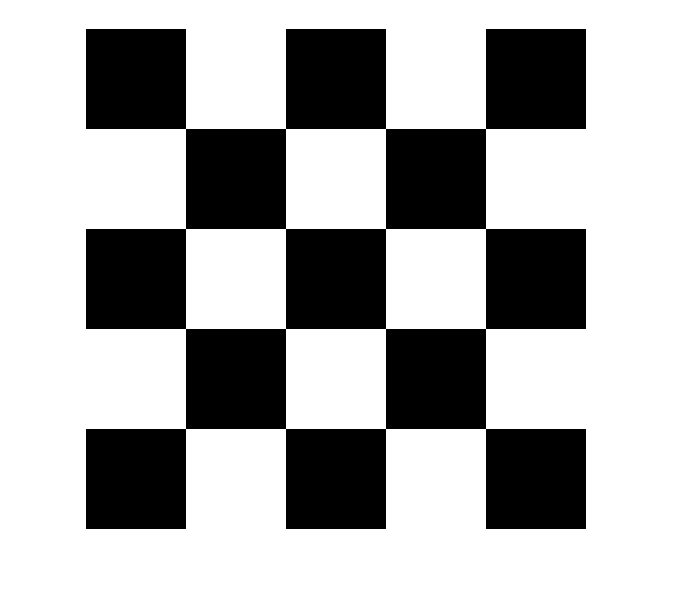
\includegraphics[width=0.5\linewidth]{images/checkerboard.png}
    \end{figure}
\subsection*{Solution}

    \begin{lstlisting}[language=Matlab]
I=imread('checkerboard.png');
FNT_SZ=28;
figure(1), imshow(I);
hold on;
[x,y]=getpts();
a=[x(1);y(1);1];
b=[x(2);y(2);1];
c=[x(3);y(3);1];
d=[x(4);y(4);1];
text(a(1),a(2),'a','FontSize',FNT_SZ,'Color','b')
text(b(1),b(2),'b','FontSize',FNT_SZ,'Color','b')
text(c(1),c(2),'c','FontSize',FNT_SZ,'Color','b')
text(d(1),d(2),'d','FontSize',FNT_SZ,'Color','b')
lab=cross(a,b); 
lad=cross(a,d); 
lac=cross(a,c); 
lcd=cross(c,d);
r1=[0;1;-1];       % Parameters of top-most row
r500=[0;1;-500];   % Parameters of bottom row
c1=[1;0;-1];       % Parameters of left-most column
c500=[1;0;-500];   % Parameters of right-most column
% Intersection between lab and the first column
x1=cross(c1,lab); 
x1=x1/x1(3); 
text(x1(1),x1(2),'x1','FontSize',FNT_SZ,'Color','b')
% Same with the right most column
x500=cross(c500,lab);
x500=x500/x500(3);
text(x500(1),x500(2),'x500','FontSize',FNT_SZ,'Color','b')
plot([x1(1),x500(1)],[x1(2),x500(2)],'LineWidth',3)
computeEuclideanAngles(lab,lac) 
computeEuclideanAngles(lab,lcd) 
computeEuclideanAngles(lab,lad) 
lambda=rand(1);
mu=1-lambda;
p= lambda*a+mu*b;
p'*lab
p=p/p(3);
text(p(1),p(2),'p','FontSize',FNT_SZ,'Color','b')
vac=cross(lab,lcd)
vac=vac/vac(3) 
vab=cross(r1,r500)
vad=cross(c1,c500)
    \end{lstlisting}

    \newpage

    \section{Cubes}
        Elaborate the following image called "simplecube-letters.png": 
        \begin{figure}[H]
            \centering
            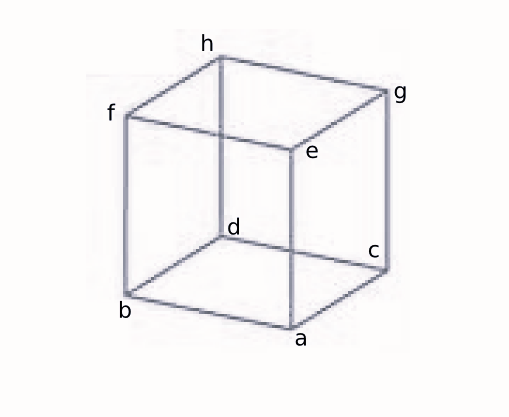
\includegraphics[width=0.5\linewidth]{images/simplecube-letters.png}
        \end{figure}
        And the following image called "buildingSmall.png": 
        \begin{figure}[H]
            \centering
            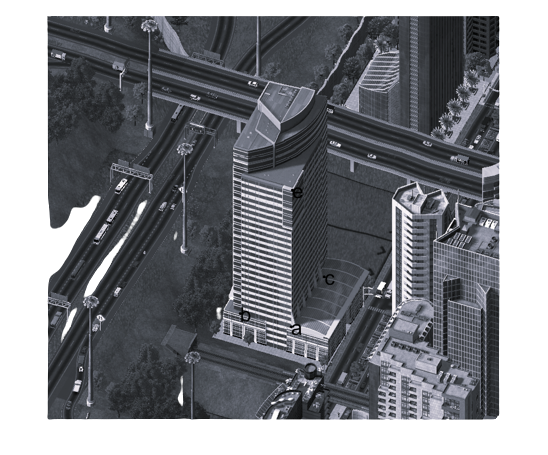
\includegraphics[width=0.5\linewidth]{images/buildingSmall.png}
        \end{figure}
    \subsection*{Solution}
        \begin{lstlisting}[language=Matlab]
figure(1),imshow(imread('simplecube-letters.png'));
figure(2),imshow(imread('buildingSmall.png'))
hold on;
[x y]=getpts
plot(x,y,'.w','MarkerSize',12,'LineWidth',3);
a=[x(1) y(1) 1]';
text(a(1),a(2),'a','FontSize',FNT_SZ,'Color','w')
b=[x(2) y(2) 1]';
text(b(1),b(2),'b','FontSize',FNT_SZ,'Color','w')
c=[x(3) y(3) 1]';
text(c(1),c(2),'c','FontSize',FNT_SZ,'Color','w')
e=[x(4) y(4) 1]';
text(e(1),e(2),'e','FontSize',FNT_SZ,'Color','w')
lab=cross(a,b)
lac=cross(a,c)
lae=cross(a,e)
lab'*a
lab'*b
lac'*a
lac'*c
lae'*a
lae'*e
linf=[0 0 1]';
dab=cross(lab,linf)
dac=cross(lac,linf)
dae=cross(lae,linf)
lbd=cross(b,dac);
lcd=cross(c,dab);
d=cross(lbd,lcd);
d=d/d(3);
plot(d(1),d(2),'.b','MarkerSize',12);
text(d(1),d(2),'d','FontSize',FNT_SZ,'Color','w')
lbf=cross(b,dae);
lcg=cross(c,dae);
ldh=cross(d,dae);
lef=cross(e,dab);
leg=cross(e,dac);
f=cross(lbf,lef);
g=cross(lcg,leg);
lfh=cross(f,dac);
h=cross(lfh,ldh);
f=f/f(3);
g=g/g(3);
h=h/h(3);
plot(f(1),f(2),'.w','MarkerSize',12,'LineWidth',3); 
text(f(1),f(2),'f','FontSize',FNT_SZ,'Color','w')
plot(g(1),g(2),'.w','MarkerSize',12,'LineWidth',3); 
text(g(1),g(2),'g','FontSize',FNT_SZ,'Color','w')
plot(h(1),h(2),'.w','MarkerSize',12, 'LineWidth',3);
text(h(1),h(2),'h','FontSize',FNT_SZ,'Color','w')
myline=[a';b';d';c';a'];
line(myline(:,1),myline(:,2),'LineWidth',5);
myline=[e';f';h';g';e'];
line(myline(:,1),myline(:,2),'LineWidth',5);
myline=[a';e'];
line(myline(:,1),myline(:,2),'LineWidth',5);
myline=[b';f'];
line(myline(:,1),myline(:,2),'LineWidth',5);
myline=[c';g'];
line(myline(:,1),myline(:,2),'LineWidth',5);
myline=[d';h'];
line(myline(:,1),myline(:,2),'LineWidth',5);
hold off
        \end{lstlisting}

\newpage

\chapter{Laboratory session II}
    \section{Affine rectification}
        Identify pairs of parallel lines in the image of a plane and get their vanishing points. Compute the vanishing line and use it to perform an affine rectification of 
        the plane.
        \begin{figure}[H]
            \centering
            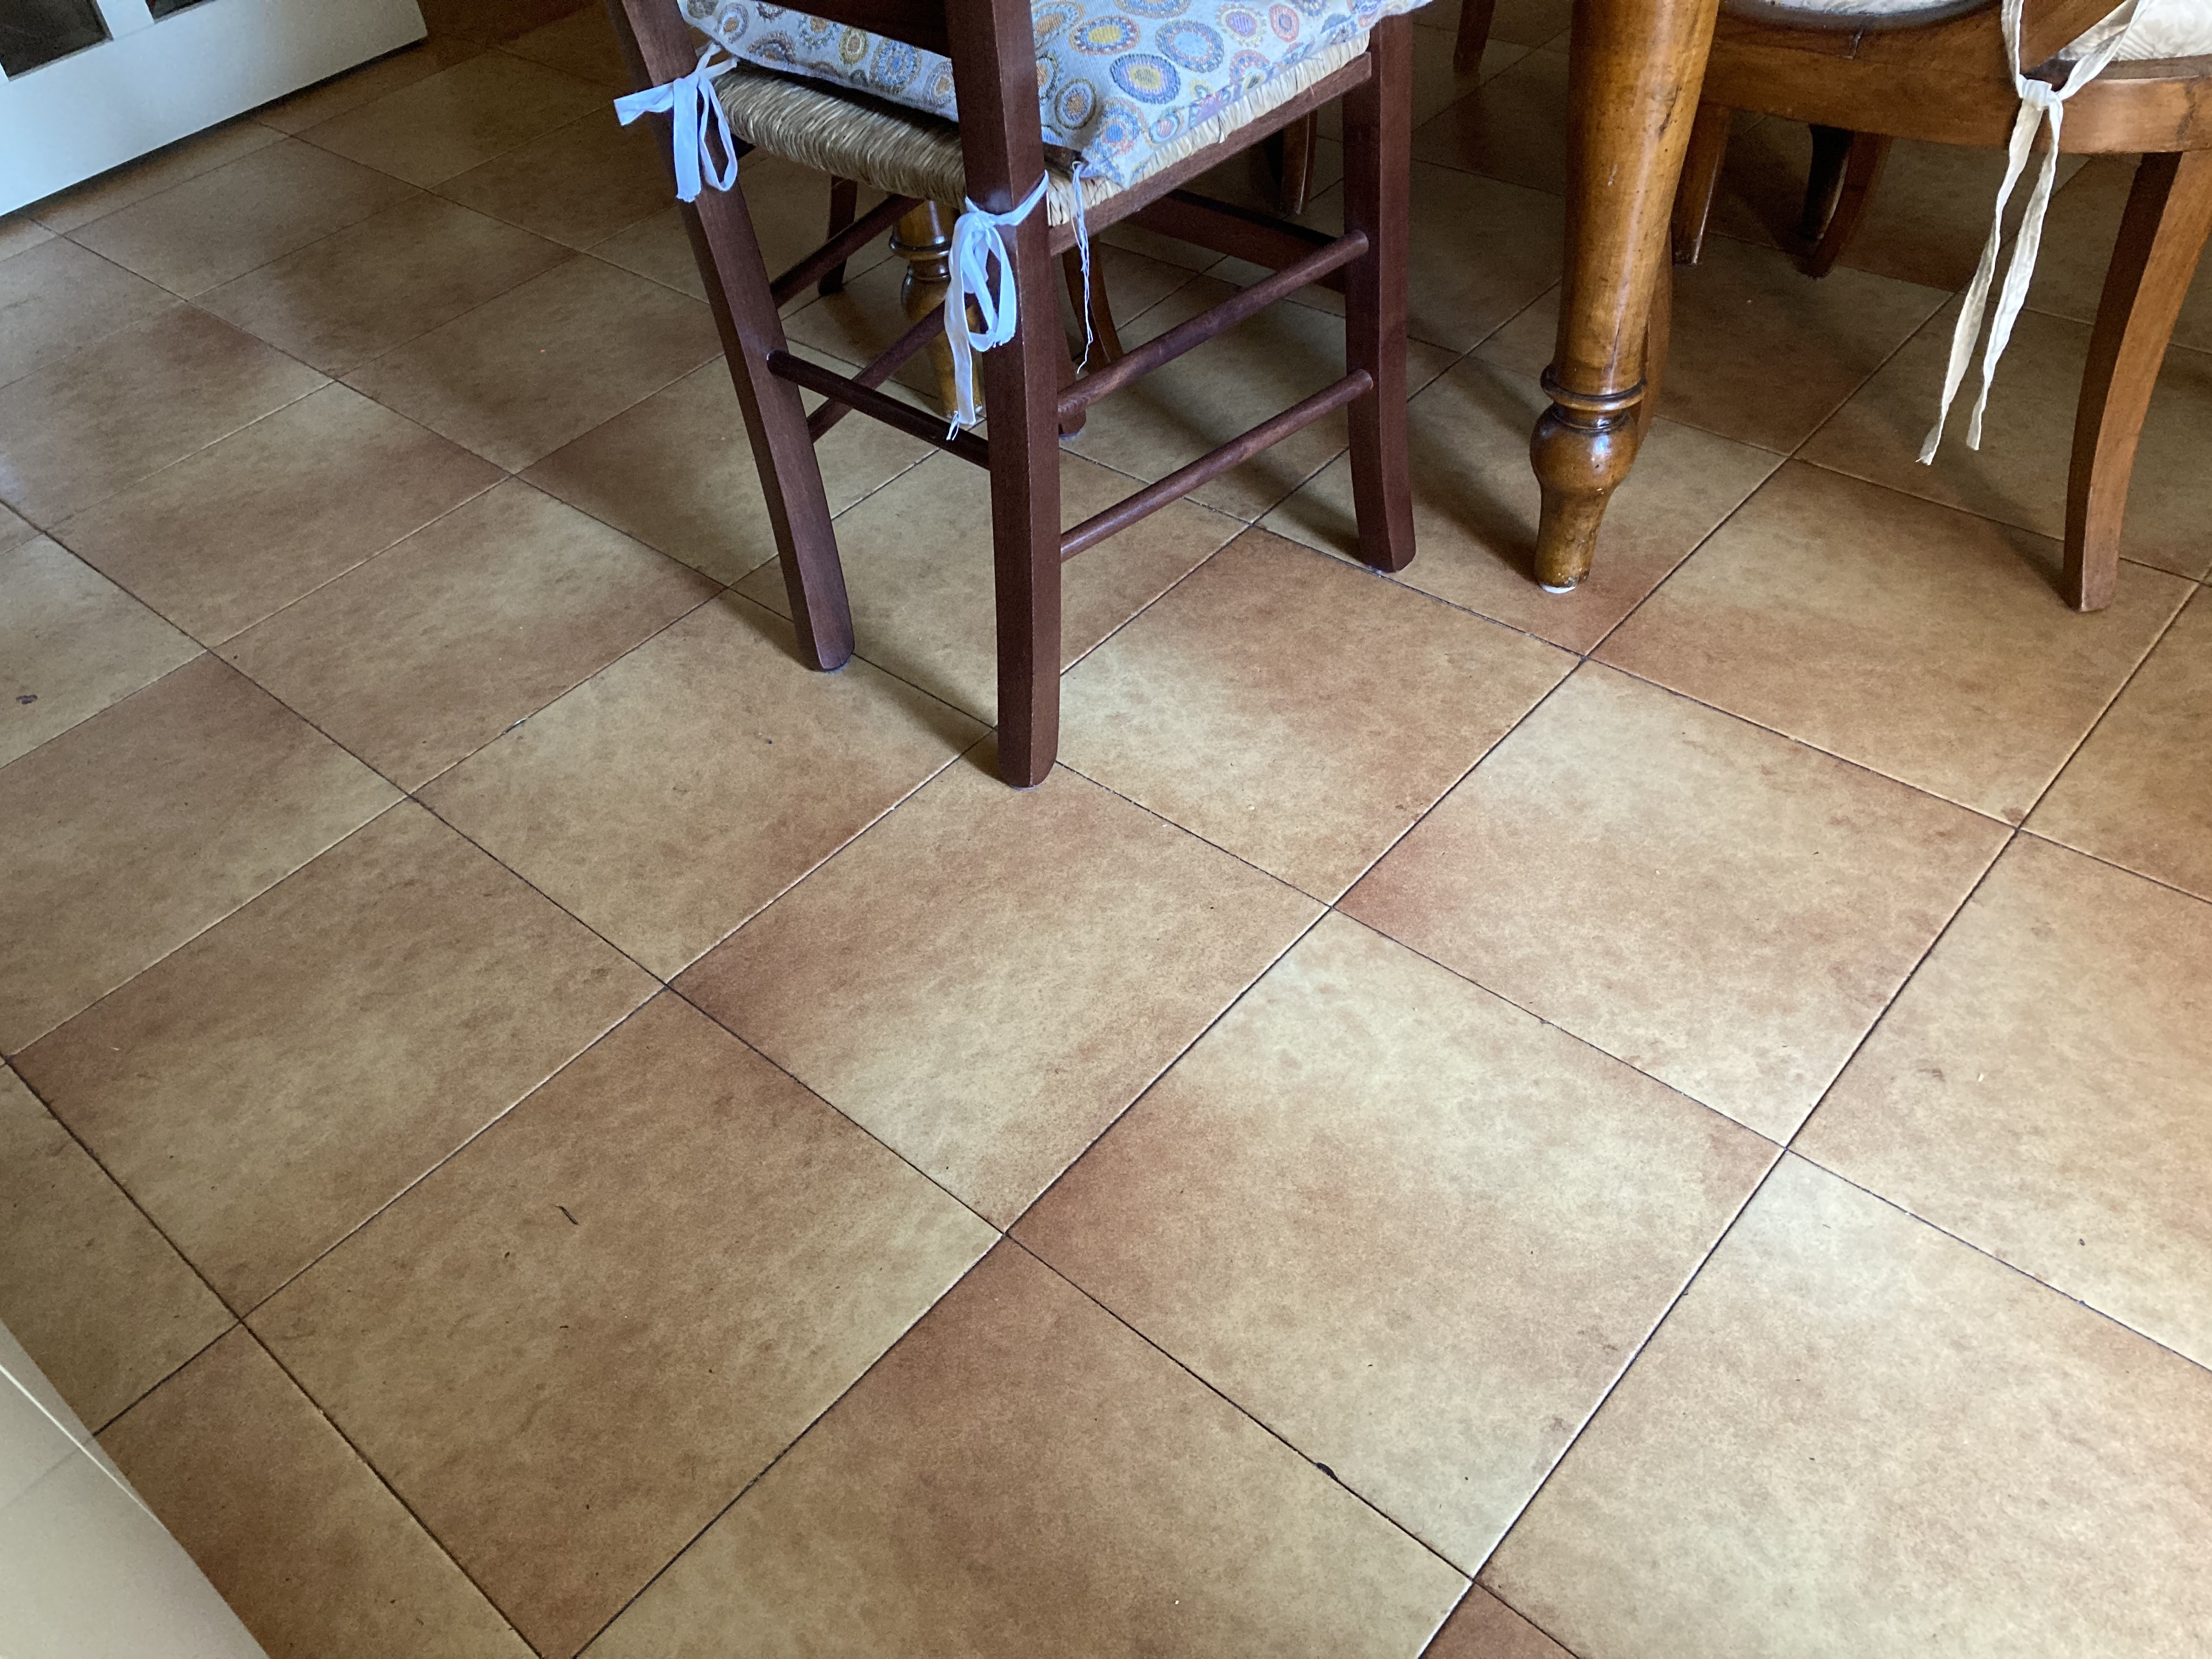
\includegraphics[width=0.75\linewidth]{images/floor.png}
        \end{figure}
    \subsection*{Solution}
        \begin{lstlisting}[language=Matlab]
clc;
clear;
% load an image of a plane
im=imread("E2_data/floor.jpg");
im=imresize(im,0.5);
% select four points
% important select the point clockwise or counterclockwise
figure;
imshow(im);
hold on;
[x,y]=getpts();
a=[x(1);y(1);1];
b=[x(2);y(2);1];
c=[x(3);y(3);1];
d=[x(4);y(4);1];
FNT_SZ=20;
text(a(1),a(2),'a','FontSize',FNT_SZ,'Color','b')
text(b(1),b(2),'b','FontSize',FNT_SZ,'Color','b')
text(c(1),c(2),'c','FontSize',FNT_SZ,'Color','b')
text(d(1),d(2),'d','FontSize',FNT_SZ,'Color','b')
% compute the lines passing through the points
lab=cross(a,b);
lbc=cross(b,c);
lcd=cross(c,d);
lda=cross(d,a);
% we can get vanishing points from pairs of parallel line 
% in closed form
v1=cross(lab,lcd);
v2=cross(lbc,lda);
% remember these have to be normalized before plotting them
v1=v1/v1(3);
v2=v2/v2(3);
% Compute the horizon (the vanishing line of the plane)
% the horizon is just the line that passes thorugh the 
% vanishing points
horizon = cross(v1,v2);
% display the result
plot([a(1),v1(1)],[a(2),v1(2)],'b');
plot([d(1),v1(1)],[d(2),v1(2)],'b');
plot([b(1),v1(1)],[b(2),v1(2)],'b');
plot([c(1),v1(1)],[c(2),v1(2)],'b');
plot([a(1),v2(1)],[a(2),v2(2)],'b');
plot([c(1),v2(1)],[c(2),v2(2)],'b');
plot([b(1),v2(1)],[b(2),v2(2)],'b');
plot([d(1),v2(1)],[d(2),v2(2)],'b');
plot([v1(1),v2(1)],[v1(2),v2(2)],'b--')
text(v1(1),v1(2),'v1','FontSize',FNT_SZ,'Color','b')
text(v2(1),v2(2),'v2','FontSize',FNT_SZ,'Color','b')
hold off
disp('Select another pair of parallel lines');
figure(gcf),
hold on;
[x,y]=getpts();
e=[x(1);y(1);1];
f=[x(2);y(2);1];
g=[x(3);y(3);1];
h=[x(4);y(4);1];
lef=cross(e,f);
lgh=cross(g,h);
v3=cross(lef,lgh);
v3=v3/v3(3);
horizon'*v3
plot([e(1),v3(1)],[e(2),v3(2)],'r');
plot([g(1),v3(1)],[g(2),v3(2)],'r');
text(v3(1),v3(2),'v3','FontSize',FNT_SZ,'Color','b');
% Given the horizon we can rectify the image
% for numerical stability it is important to scale the coefficient
% of the horizon
horizon=horizon./norm(horizon);
H=[eye(2),zeros(2,1);horizon(:)'];
H=det(H)*H;
fprintf('The vanishing line is mapped to:\n');
disp(inv(H)'*horizon);
% rectify the image
t=maketform('projective',H');
J=imtransform(im,t);
figure;
imshow(J);
        \end{lstlisting}

    \newpage 
    
    \section{Affine measurements}
    This code demonstrates the estimation of vanishing points and vanishing lines to take affine measurements from an image. Specifically this code allows to estimate the 
    height of an object standing on the ground, provided:
    \begin{itemize}
        \item The height of a reference object standing on the ground. 
        \item A vertical vanishing point. 
        \item The vanishing line of the ground
    \end{itemize}
    \begin{figure}[H]
        \centering
        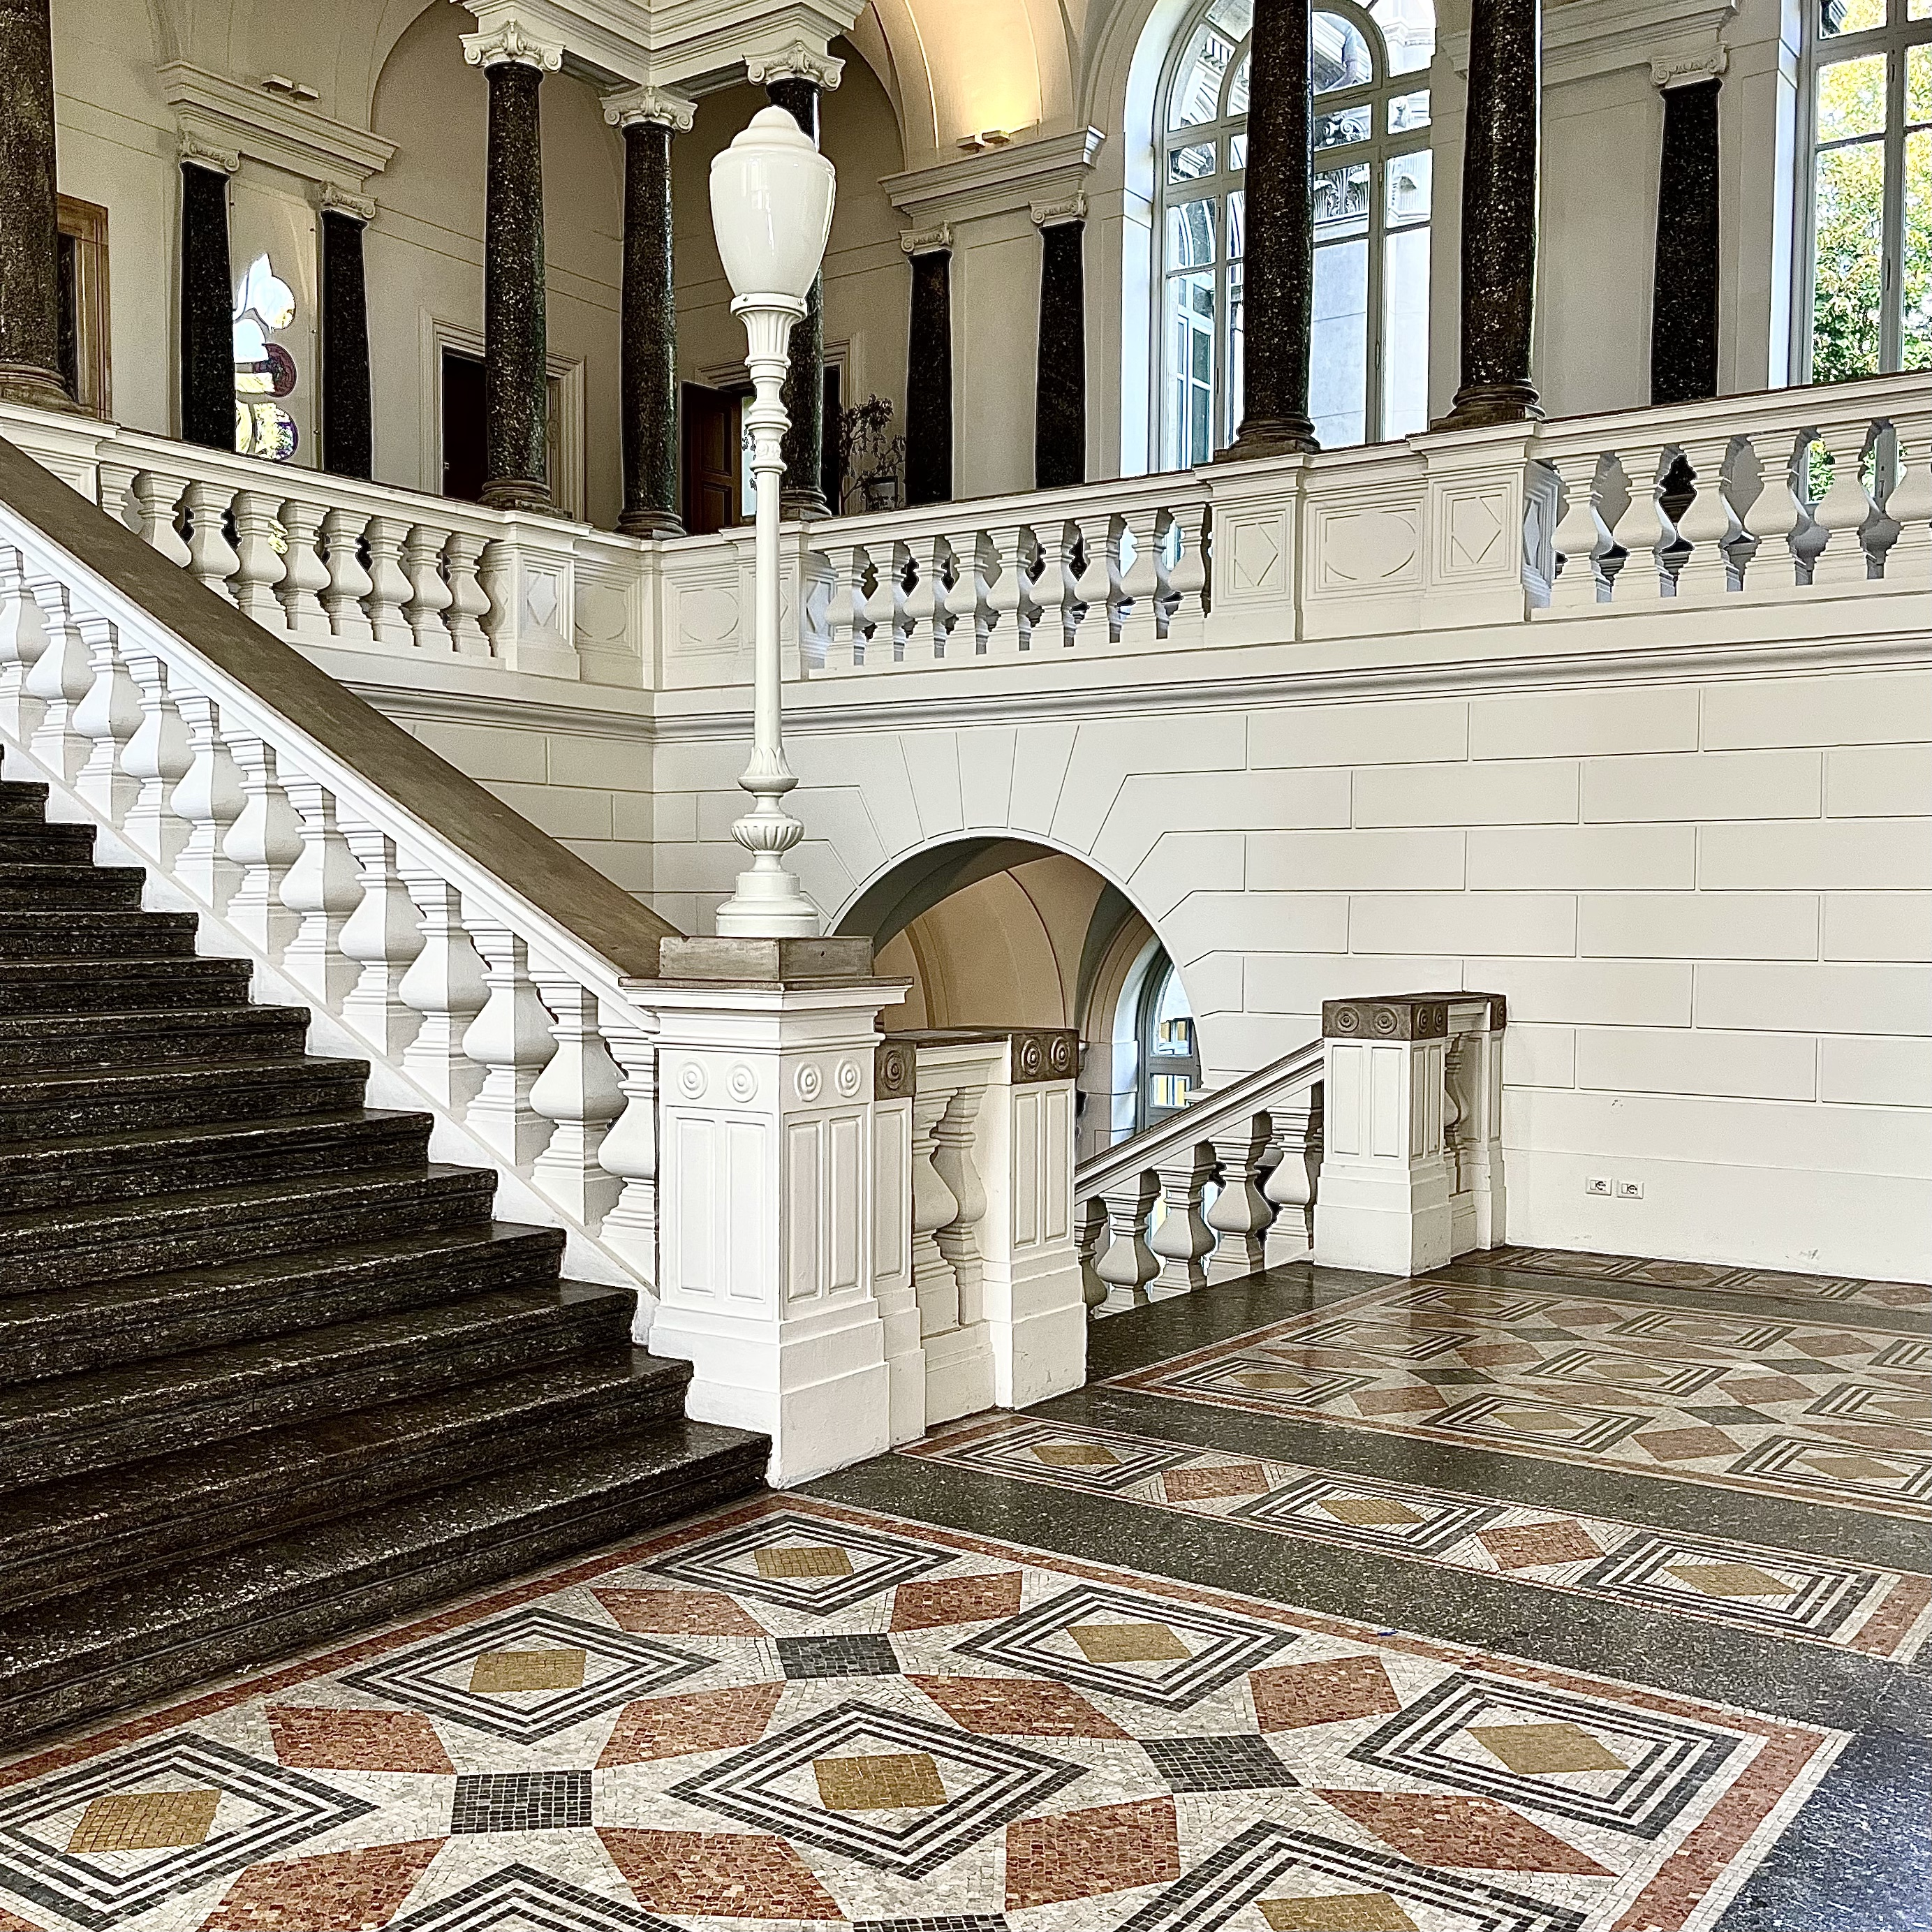
\includegraphics[width=0.75\linewidth]{images/poli2.png}
    \end{figure}
    \subsection*{Solution}
        \begin{lstlisting}
clear 
clc 
% load image
im = imread('poli2.jpg');
im = imresize(im,0.6);
figure(1);
imshow(im);
% draw vertical segments in the image 
numSegments=4; 
verticalLines=nan(numSegments,3);
endPoints=nan(2,numSegments); 
count=1;
while(count<=numSegments)
    figure(1);
    title(['Draw',num2str(numSegments),'vertical segments:step',num2str(count)]);
    seg=drawline('Color','b');
    % convert the end points of the segments into the coefficients 
    % of the line
    endPoints(:,count)=seg.Position(1,:)';
    % switch to homoegeous coordinates
    a=[seg.Position(1,:)';1];
    b=[seg.Position(2,:)';1];
    % get the parameters of the line
    l= cross(a,b);
    l=l./norm(l);
    verticalLines(count,:)=l';
    count=count+1;
end
fprintf('Press enter to continue\n');
pause
% compute vanishing points from pairs of images
v1 = cross(verticalLines(1,:),verticalLines(2,:));
v1 = v1./v1(3);
v2 = cross(verticalLines(3,:),verticalLines(4,:));
v2 = v2./v2(3);
v3 = cross(verticalLines(1,:),verticalLines(4,:));
v3 = v3./v3(3);
figure;
%imshow(im);
hold all;
plot(v1(1),v1(2),'ko','MarkerSize',10,'MarkerFaceColor','r');
line([endPoints(1,1),v1(1)],[endPoints(2,1),v1(2)],'Color', 
'r','LineWidth',3);
line([endPoints(1,2),v1(1)],[endPoints(2,2),v1(2)],'Color',
    'r','LineWidth',3);
plot(v2(1),v2(2),'ko','MarkerSize',10,'MarkerFaceColor','g');
line([endPoints(1,3),v2(1)],[endPoints(2,3),v2(2)],'Color', 
    'g','LineWidth',3);
line([endPoints(1,4),v2(1)],[endPoints(2,4),v2(2)],'Color',
    'g','LineWidth',3);
plot(v3(1),v3(2),'ko','MarkerSize',10,'MarkerFaceColor','c');
line([endPoints(1,1),v3(1)],[endPoints(2,1),v3(2)],'Color','
    c','LineWidth',3);
line([endPoints(1,4),v3(1)],[endPoints(2,4),v3(2)],'Color',
    'c','LineWidth',3);
title('Vertical vanishing point');
% we can minimize an algebraic error
[u,s,v]=svd(verticalLines);
V_vert=v(:,end);
V_vert=V_vert/V_vert(3);
figure(gcf);
hold all;
plot(V_vert(1),V_vert(2),'bo','MarkerSize',30,
    'MarkerFaceColor','b');
f=2;
numSegments=4;
parallelLines=cell(f,1);
fprintf(['Draw',num2str(f),'families of parallel segments\n']);
col='rgm';
figure;
imshow(im)
for i=1:f
    count=1;
    parallelLines{i}=nan(numSegments,3);
    while(count<=numSegments)
        figure(gcf);
        title(['Draw',num2str(numSegments),'segments:step',
              num2str(count)]);
        seg=drawline('Color',col(i));
        endPoints=seg.Position;
        a=[endPoints(1,:)';1];
        b=[endPoints(2,:)';1];
        l=cross(a,b);
        l=l./norm(l); 
        parallelLines{i}(count,:)=l;
        count=count+1;
    end
    fprintf('Press enter to continue\n');
    pause
end
% compute the vanishing points
V=nan(3,f);
for i=1:f
    [u,s,v]=svd(parallelLines{i});
    V(:,i)=v(:,end);
    V(:,i)=V(:,i)./V(3,i);
end
% compute the horizon
horizon=cross(V(:,1),V(:,2));
figure;
hold all;
for i=1:f
    plot(V(1,i),V(2,i),'o','Color',col(i),'MarkerSize',20,
        'MarkerFaceColor',col(i));
end
line(V(1,:),V(2,:),'Color','b','Linewidth',4)
%hold all;
imshow(im);
figure;
imshow(im);
title('select a reference object')
seg1=drawline('Color','c');
seg2=drawline('Color','m');
b1=[seg1.Position(1,:)';1];
t1=[seg1.Position(2,:)';1];
b2=[seg2.Position(1,:)';1];
t2=[seg2.Position(2,:)';1];
% dispaly the selected points
TXT_OFFSET=20;
figure;
imshow(im);
hold all;
plot(b1(1),b1(2),'c.','MarkerSize',20,'LineWidth',5);
text(b1(1)+TXT_OFFSET,b1(2),'b1','FontSize',30,'Color','c');
plot(t1(1),t1(2),'.','Color','c','MarkerSize',20,'LineWidth',5);
text(t1(1)+TXT_OFFSET,t1(2),'t1','FontSize',30,'Color','c');
plot(b2(1),b2(2),'m.','MarkerSize',20,'LineWidth',5);
text(b2(1)+TXT_OFFSET,b2(2),'b2','FontSize',30,'Color','m');
plot(t2(1),t2(2),'m.','MarkerSize',20,'LineWidth',5);
text(t2(1)+TXT_OFFSET,t2(2),'t2','FontSize',30,'Color','m');
% compute the relative distance
u=cross(cross(b1,b2),horizon);
u=u./u(3);
l2=cross(V_vert,b2);
t1_tilde=cross(cross(t1,u),l2);
t1_tilde=t1_tilde/t1_tilde(3);
% compute the distance from b2
dist_t1_tilde=norm(t1_tilde-b2);
dist_t2=norm(t2-b2);
dist_v=norm(V_vert-b2);
% compute 1D projective transfomration mapping the vanishing 
% point to infinity
H=[1 0; 1 -dist_v];
H*[dist_v;1]
% compute the distance ratio
d1_d2_ratio=dist_t1_tilde*(dist_v-dist_t2)/
   (dist_t2*(dist_v-dist_t1_tilde));
lenght1=122;
lenght2=lenght1/d1_d2_ratio
TXT_OFFSET=20;
FNT_SIZE=30;
c1='w';
c2='m';
c3='b';
figure;
imshow(im);
hold all;
line(V(1,:),V(2,:),'Color',c3,'Linewidth',2);
line([b1(1),t1(1)],[b1(2),t1(2)],'Color',c1,'Linewidth',2);
line([b2(1),t2(1)],[b2(2),t2(2)],'Color',c2,'Linewidth',2);
plot(b1(1),b1(2),'.','Color',c1,'MarkerSize',20,'LineWidth',2);
text(b1(1)+TXT_OFFSET,b1(2),'b1','FontSize',FNT_SIZE,'Color',c1);
plot(t1(1),t1(2),'.','Color',c1,'MarkerSize',20,'LineWidth',5);
text(t1(1)+TXT_OFFSET,t1(2),'t1','FontSize',FNT_SIZE,'Color',c1);
plot(b2(1),b2(2),'.','Color',c2,'MarkerSize',20,'LineWidth',5);
text(b2(1)+TXT_OFFSET,b2(2),'b2','FontSize',FNT_SIZE,'Color',c2);
plot(t2(1),t2(2),'.','Color',c2,'MarkerSize',20,'LineWidth',5);
text(t2(1)-TXT_OFFSET,t2(2)+TXT_OFFSET,'t2','FontSize',30,
    'Color',c2);
plot(u(1),u(2),'o','Color',c3,'Markersize',20,'MarkerFaceColor',c3)
text(u(1)+TXT_OFFSET,u(2),'u','FontSize',FNT_SIZE,'Color',c3);
plot(t1_tilde(1),t1_tilde(2),'d','Color',c3,'MarkerSize',
    10,'LineWidth',5,'MarkerFaceColor', c3);
text(t1_tilde(1)+TXT_OFFSET,t1_tilde(2),'t1 tilde','FontSize',30,'Color',c3);
line([b2(1),u(1)],[b2(2),u(2)],'Color',c3,'Linewidth',2);
line([t1_tilde(1),u(1)],[t1_tilde(2),u(2)],
    'Color',c3,'Linewidth',2);
hold on;
c1='r';
figure;
imshow(im);
hold all;
line([b1(1),t1(1)],[b1(2),t1(2)],'Color',c1,'Linewidth',2);
text(0.5*(b1(1)+t1(1)),0.5*(b1(2)+t1(2)),num2str(lenght1,"%i"),
    'FontSize',FNT_SIZE,'Color',c1);
line([b2(1),t2(1)],[b2(2),t2(2)],'Color',c1,'Linewidth',2);
text(0.5*(b2(1)+t2(1)),0.5*(b2(2)+t2(2)),num2str(round(lenght2)),
    'FontSize',FNT_SIZE,'Color',c1);
        \end{lstlisting} 

        \newpage 
    
        \section{Horizon}
        Identify pairs of equi-spaced parallel planar lines in an image. Compute the vanishing line and use it to perform an affine rectification of the plane.
        \begin{figure}[H]
            \centering
            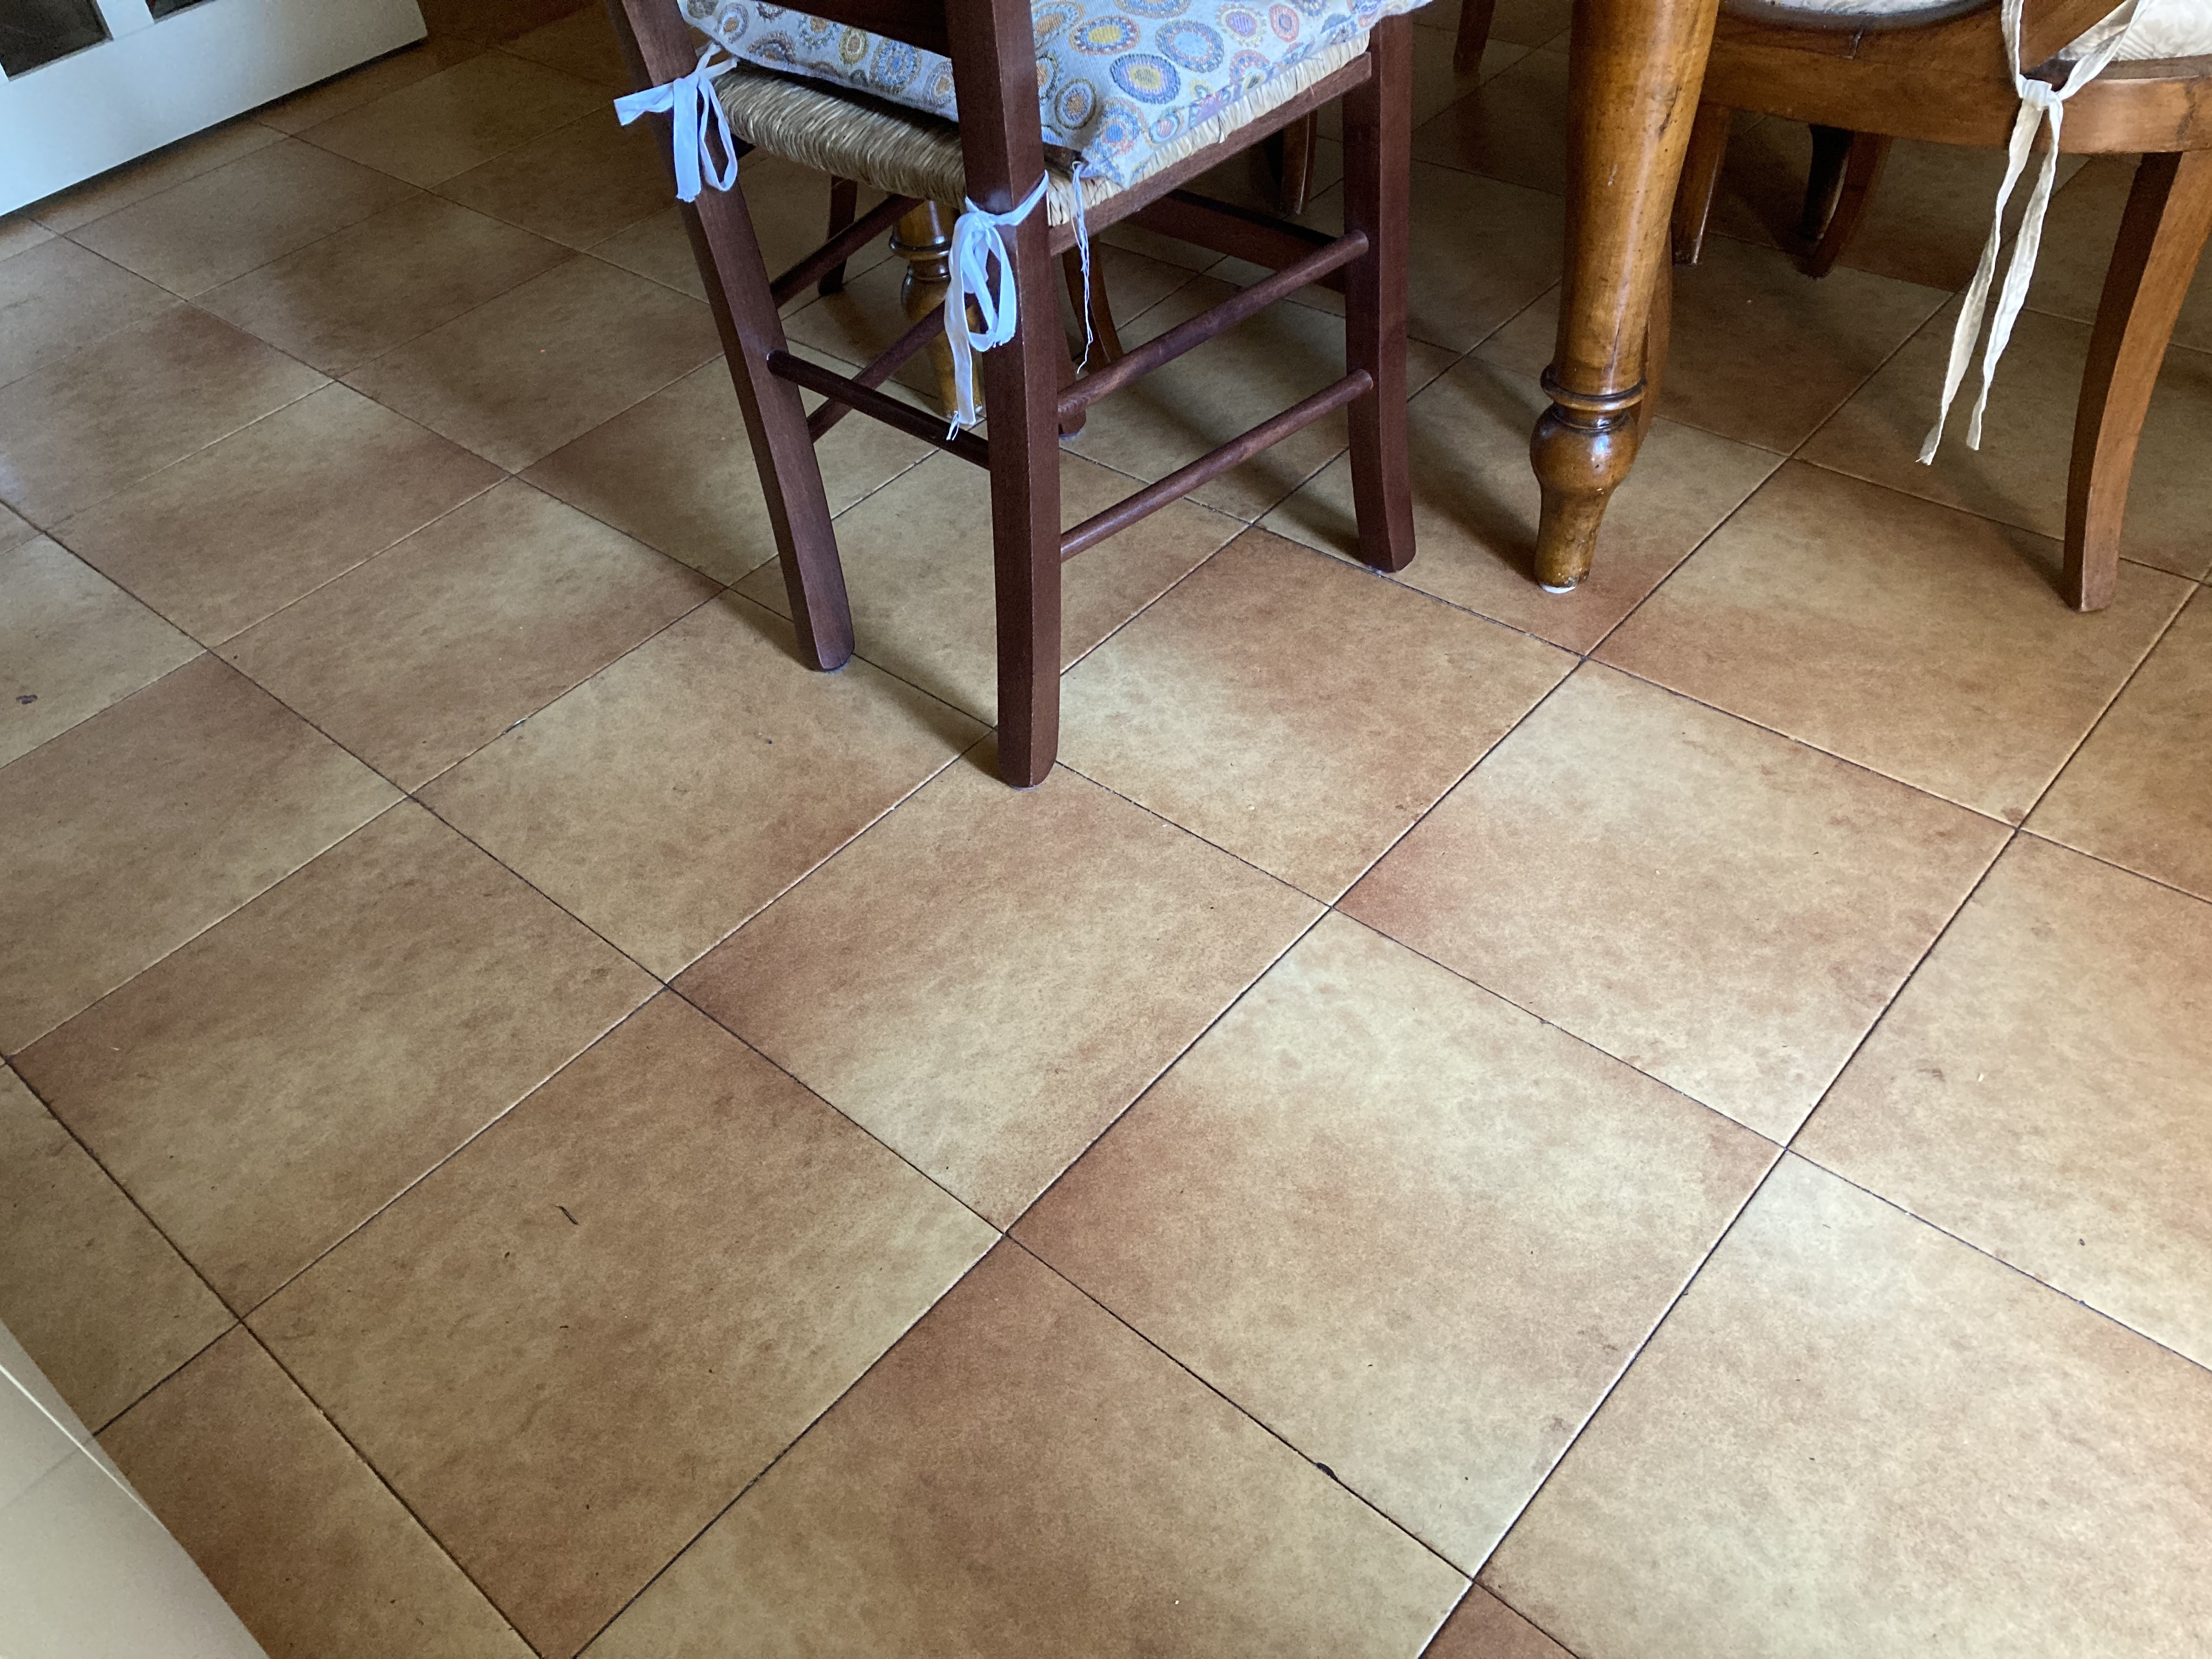
\includegraphics[width=0.75\linewidth]{images/floor.png}
        \end{figure}
        \subsection*{Solution}
            \begin{lstlisting}
im=imread("E2_data/floor.jpg");
im=imresize(im,0.5);
figure;imshow(im);
fori=1:3
    seg{i}=drawline('Color','b');
    %convertthesegmentstoline
    a=[seg{i}.Position(1,:)';1];
    b=[seg{i}.Position(2,:)';1];
    %gettheparametersoftheline
    lines{i}=cross(a,b);
end
l0=lines{1};
l1=lines{2};
l2=lines{3};
l=(cross(l0,l2)'*cross(l1,l2))*l1
  +2*(cross(l0,l1)'*cross(l2,l1)*l2);
horizon=l./norm(l);
P1=[0;-horizon(3)/horizon(2)];
P2=[size(im,2);-(horizon(1)*size(im,2)+horizon(3))/horizon(2)];
figure(gcf);
holdon
line([P1(1),P2(1)],[P1(2),P2(2)],'Linewidth',4,'Color','b');
horizon=horizon./norm(horizon);
H=[eye(2),zeros(2,1);horizon(:)'];
H=det(H)*H;
fprintf('Thevanishinglineismappedto:\n');
disp(inv(H)'*horizon);
t=maketform('projective',H');
J=imtransform(im,t);
figure;
imshow(J);
            \end{lstlisting} 


\end{document}